\documentclass[a4paper,12pt]{article} % This defines the style of your paper

\usepackage[top = 2.5cm, bottom = 2.5cm, left = 2.5cm, right = 2.5cm]{geometry} 

\usepackage[T1]{fontenc}
\usepackage[utf8]{inputenc}

\usepackage{graphicx} 

% The default setting of LaTeX is to indent new paragraphs.
\usepackage{setspace}
\setlength{\parindent}{0in}

% Package to place figures where you want them.
\usepackage{float}

% The fancyhdr package let's us create nice headers.
\usepackage{fancyhdr}

% Code blocks with syntax highlight package
\usepackage{listings}
\usepackage{color}

\definecolor{comments}{rgb}{0.25,0.5,0.5}
\definecolor{keywords}{rgb}{0.016,0.51,0.016}
\definecolor{strings}{rgb}{0.776,0.294,0.294}

\lstset{ %
  backgroundcolor=\color{white},   % choose the background color
  basicstyle=\footnotesize,        % size of fonts used for the code
  breaklines=true,                 % automatic line breaking only at whitespace
  captionpos=b,                    % sets the caption-position to bottom
  commentstyle=\color{comments},    % comment style
  escapeinside={\%*}{*)},          % if you want to add LaTeX within your code
  keywordstyle=\color{keywords},       % keyword style
  stringstyle=\color{strings},     % string literal style
}

%%%%%%%%%%%%%%%%%%%%%%%%%%%%%%%%%%%%%%%%%%%%%%%%
% 3. Header (and Footer)
%%%%%%%%%%%%%%%%%%%%%%%%%%%%%%%%%%%%%%%%%%%%%%%%

\pagestyle{fancy} % With this command we can customize the header style.

\fancyhf{} % This makes sure we do not have other information in our header or footer.

\lhead{\footnotesize PDS: Proyecto final}% \lhead puts text in the top left corner. \footnotesize sets our font to a smaller size.

%\rhead works just like \lhead (you can also use \chead)
\rhead{\footnotesize César Augusto Montoya Ocampo (1036681523)} %<---- Fill in your lastnames.

% Similar commands work for the footer (\lfoot, \cfoot and \rfoot).
% We want to put our page number in the center.
\cfoot{\footnotesize \thepage} 

\begin{document}

\thispagestyle{empty} % This command disables the header on the first page. 

\begin{tabular}{p{15.5cm}} % This is a simple tabular environment to align your text nicely 
{\large \bf Procesamiento digital de señales} \\
Universidad de Antioquia \\ 2023-1  \\ Proyecto final \\
\hline % \hline produces horizontal lines.
\\
\end{tabular} % Our tabular environment ends here.

\vspace*{0.3cm} % Now we want to add some vertical space in between the line and our title.

\begin{center} % Everything within the center environment is centered.
	{\Large \bf Filtros adaptativos} % <---- Don't forget to put in the right number
	\vspace{2mm}
	
        % YOUR NAMES GO HERE
	{\bf César Augusto Montoya Ocampo (1036681523)} % <---- Fill in your names here!
		
\end{center}  

\vspace{0.4cm}

El principio de operación de un filtro adaptativo son sus características variables en el tiempo autoajustables. Un filtro adaptativo usualmente toma la forma de un filtro FIR, con un algoritmo de adaptación que continuamente actualiza los coeficientes del filtro, tal que la señal de error se minimiza de acuerdo a cierto criterio. La señal de error usualmente es derivada de alguna manera desde diagrama de flujo de la aplicación, tal que sea una medida de qué tan cerca el filtro está del óptimo. [1]

\begin{figure}[H]
    \centering % Centers Graphic
    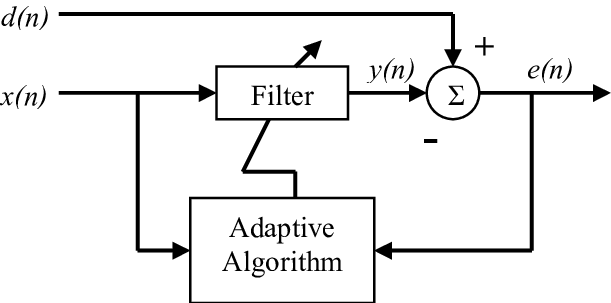
\includegraphics[width=0.8\textwidth]{block-diagram.png} 
    \caption{Diagrama de bloques de un filtro adaptativo genérico.}
\end{figure}

\begin{center}
    \section*{LMS (Least Mean Squares)}
\end{center}

El algoritmo de los mínimos cuadrados medios es extremadamente popular por su simplicidad y baja complejidad computacional. El algoritmo está basado en el método de gradiente descendiente, pero es aún más simple ya que solo ejecuta una iteración por muestra, y además, calcula solo un estimado del vector gradiente por cada muestra, los coeficientes del filtro se calculan mediante la siguiente ecuación.

\begin{equation}
    w_{n+1}(i) = w_n (i) + 2 \mu e_n x_{n-i}
\end{equation}

La variable $w$ son los coeficientes del filtro, que se actualizan con cada iteración del algoritmo, la variable $x$ es la señal de entrada del filtro, mientras que $y$ es la salida del filtro, la cual se utiliza para calcular el error en cada iteración e ir reduciendo su valor. El parámetro $\mu$ es una constante que regula la estabilidad y rapidez de convergencia, para calcular el valor del error se usa:

\begin{equation}
    e_n = d_n - \sum\limits_{i=0}^{N-1} w(i) \cdot x_{n-i}
\end{equation}

\begin{enumerate}
    \item Escriba un programa que cargue el archivo \verb|voices.wav| el cual contiene un audio con diversas voces, grafique la señal, nombrando los ejes de manera adecuada y poniendo un título respectivo a la gráfica, finalmente reproduzca el audio.

    \item Escriba un programa que cargue el archivo \verb|rock.wav| el cual contiene una pista musical, grafique la señal, nombrando los ejes de manera adecuada y poniendo un título respectivo a la gráfica, finalmente reproduzca el audio.

    \item Realice la tarea de combinar los dos audios, asegurándose de que terminen al mismo tiempo sin alterar la longitud del audio más largo, reproduzca el resultado ¿Logra distinguir ambos audios?

    \item Grafique el espectro de los audios por separado ¿Qué filtro utilizaría para intentar separar la voz del audio?

    \item Según su respuesta al numeral anterior implemente un filtro FIR con esas características, grafique la forma de onda y el espectro del resultado del filtro, reproduzca el audio filtrado ¿Fue posible remover la música usando este filtro? Para implementar el filtro puede utilizar una de las siguientes funciones.

    \begin{lstlisting}[language=python]
    def low_pass_filter(fs, cutoff_hz, roll_off, ripple_dB):
        nyq_rate = fs / 2.0
        width = roll_off/nyq_rate
        N, _ = kaiserord(ripple_dB, width)
        taps = firwin(N, cutoff_hz/nyq_rate, pass_zero="lowpass")
        return taps

    def high_pass_filter(fs, cutoff_hz, roll_off, ripple_dB):
        nyq_rate = fs / 2.0
        width = roll_off/nyq_rate
        N, _ = kaiserord(ripple_dB, width)
        taps = firwin(N, cutoff_hz/nyq_rate, pass_zero="highpass")
        return taps
    
    # Para aplicar el filtro se puede usar lfilter:
    taps = low_pass_filter(44100, 1500, 200, 60)
    fir_filtered = lfilter(taps, 1.0, x)
    \end{lstlisting}

    \item Utilice un filtro LMS para filtrar la señal combinada, como parámetro \verb|x| use la señal combinada, como parámetro \verb|d| use la señal de voz individual, y como parámetro \verb|mu| use 0.1, grafique el espectro de las voces originales, y del resultado de los dos filtros para poder comparar, reproduzca el resultado, según el espectro, y el audio resultante ¿Qué resultado se parece más al original? ¿Fue posible aislar las voces? ¿Por qué algunas voces resultaron distorsionadas y otras no? Puede ayudarse de la siguiente función para implementar el filtro LMS.
    \clearpage
    \begin{lstlisting}[language=python]
        def lms(x, d, N=4, mu=0.1):
            nIters = min(len(x), len(d)) - N
            # Copia de la senal
            u = np.zeros(N)
            # Coeficientes del filtro
            w = np.zeros(N)
            # Salida del filtro
            y = np.zeros(nIters)
            # Error estimado
            e = np.zeros(nIters)
            for n in range(nIters):
                # Tomar una copia de la senal
                u[1:] = u[:-1]
                u[0] = x[n]
                # Calcular la salida del filtro
                y[n] = np.dot(u, w)
                # Calcular el error estimado
                e_n = d[n] - y[n]
                # Actualizar los pesos del filtro
                w = w + 2*mu * e_n * u
                e[n] = e_n
            return y
    \end{lstlisting}
        
    \item Para poder observar mejor el comportamiento del filtro, aplique el filtro al audio combinado para los valores de $\mu$ de 0.001, 0.01, 0.1 y 0.2. Determine de qué manera influye este parámetro en el algoritmo.
\end{enumerate}

\section*{Conclusiones}

Tómese el tiempo de escribir conclusiones generales de la práctica realizada, estas deben ser basadas en lo trabajado, y en caso de referenciar algún artículo externo deberá citarlo.

\section*{Referencias}
[1] "EEE305 - Digital Signal Processing". https://www.staff.ncl.ac.uk/oliver.hinton/eee305/

\end{document}
